\documentclass{article}
\usepackage{tccml_iclr2025_conference}
\usepackage{graphicx}
\usepackage{url}
\usepackage{caption}
\usepackage{hyperref} % Load hyperref after natbib
\usepackage{amsmath}
\usepackage{colortbl} % For coloring table cells
\usepackage{sidecap} % For side captions
\usepackage{ragged2e}

% prev title: Exploring Multi-Model Ensembling Methods to Improve on Deep Learning Based Smoke Detection
\title{Improving Deep Learning-Based Wildfire\\ Smoke Plume Detection with a Multi-Model\\ Ensemble Approach}
\author{Author Name \\
Institution \\
\texttt{email@example.com}
}
\iclrfinalcopy

% % \setlength{\parskip}{2pt}
% \setlength{\textfloatsep}{10pt plus 0pt minus 0pt}
% \setlength{\floatsep}{10pt plus 0pt minus 0pt}
% \setlength{\intextsep}{10pt plus 0pt minus 0pt}

\begin{document}
\maketitle
\begin{abstract}
With the increasing frequency and severity of wildfires, there is an urgent need for effective and rapid wildfire and smoke detection tools. Recent advancements in computer vision have demonstrated the potential of deep learning models, particularly neural networks, to automate the partitioning of high-resolution images into labelled segments. However, single-model approaches can struggle with generalization and accuracy in diverse conditions. To address these challenges, we create an ensemble of deep learning models to produce more accurate annotations of wildfire smoke plumes and their relative density (light, medium, heavy) in Geostationary Operational Environmental Satellite imagery. Our results indicate that ensemble techniques can improve performance compared to using a single model. This work builds multi-model ensembles that are expected to support fire and hazard management by being able to automate the monitoring of smoke in real-time from satellite imagery. Broadly, this will be a valuable tool for air quality and fire hazard management in the face of worsening wildfires.
\end{abstract}

\section{Introduction}
Increased wildfire activity in recent years has led to a rise in smoke and particulate matter in the atmosphere, posing greater risks of respiratory illnesses and other air quality-induced health issues \citep{wildfire-risk}. Effective and timely wildfire and smoke detection tools are thus essential for supporting hazard management and mitigating risks to human health. 

The National Oceanic and Atmospheric Administration (NOAA) Geostationary Operational Environmental Satellites (GOES) provide high spatial and temporal resolution imagery of North America \citep{GOESbook}, which can be leveraged to detect the presence and density of smoke plumes. The NOAA Hazard Mapping System (HMS) Fire and Smoke Product currently relies on human analysts to annotate the presence of smoke over North America using GOES imagery \citep{hms}. However, this product is limited by the availability of human analysts and their time. Specifically, annotations are outputted only once to several times a day and usually have a delay between smoke occurance and the annotation. To address these limitations, we are leveraging advancements in deep learning to automate the detection of smoke from GOES imagery in real-time. Deep learning models, particularly encoder-decoder neural networks, have shown promise in automating the semantic segmentation (labelling images on a pixel-wise basis with multiple classes) of high-resolution images \citep{cv-segmentation-review}. By automating this task, we can enable more frequent and consistent detection of smoke plumes.

This proposal focuses on enhancing the capability of deep learning models to detect smoke through the use of multi-model ensemble techniques. It has been shown for classification tasks that ensemble methods, which combine the predictions of multiple classifiers, can often perform better than a single classifier \citep{ensemble-ml}. Particularly, utilizing a diverse set of classifiers in an ensemble is important to achieve the improvement in performance \citep{ensemble-diversity}. Furthermore, when using neural networks, combining the predictions of multiple independently-trained models can improve generalization and detection accuracy \citep{nn-ensemble}, \citep{nn-ensemble2}, \citep{nn-error-ens}. This approach aims to provide a more reliable and accurate tool for real-time monitoring of smoke, ultimately informing fire and hazard management efforts and contributing to climate resilience and adaptation strategies.
% \citep{nn-error-ens} demonstrated the importance of the neural networks having independent errors, or "error diversity" for the ensemble to succeed. it also provided a mathematical basis (clustering of errors) for designing ensembles that contain error diversity between the models.
% \section{Related Work}
\section{Data and Methods}
The dataset we use consists of 183,672 samples, each with three spectral channels (C01-C03) of GOES imagery paired with HMS smoke annotations (pixel-wise labels of smoke density of light, medium, or heavy) for a specific time and location. The data spans 2018-2024, and we use 2023 for validation and 2022 for testing, with the remaining years used for training. 

We utilize a variety of pre-developed encoder-decoder architectures that were designed for semantic segmentation contained within the Segmentation Models Pytorch library \citep{semantic}. These architectures include different features such as multi-scale fields-of-view and precise boundary detection \citep{dlv3p}, \citep{PAN}, \citep{UNetpp}, which are important for accurately detecting smoke plumes that can vary in size. Additionally, we select the best-performing single architecture and trained it with 12 different seeds to generate different initial random weights. These models are trained independently for 24 hours on 8 Nvidia P100 GPUs using the Adam optimizer, a learning rate of 1e-3, a binary cross entropy loss function, and batch size of 128. After training, each model is selected based on its best validation Intersection over Union (IoU) score (Equation \ref{overall_iou}) which quantifies the alignment between the model prediction ($ y^*_{i} $) and the ground truth ($y_{i}$).
\begin{equation} \label{overall_iou}
    \text{IoU}_{\text{overall}} = {\sum\limits_{i=\text{light}}^{\text{heavy}}|y_{i}\cap y^*_{i}|} \div {\sum\limits_{i=\text{light}}^{\text{heavy}}|y_{i}|\cup|y^*_{i}|}
\end{equation}
The ensemble method we are using is an unweighted average of the model outputs\citep{nn-ensemble2}. This ensemble framework is shown in Figure \ref{fig:ensemble_framework}. To explore how performance improves with a variety of model combinations, we vary the number of ensemble members (1-12 models) for both combinations of model architectures and initial seeds.
% \begin{figure}[h]
%     \centering
%     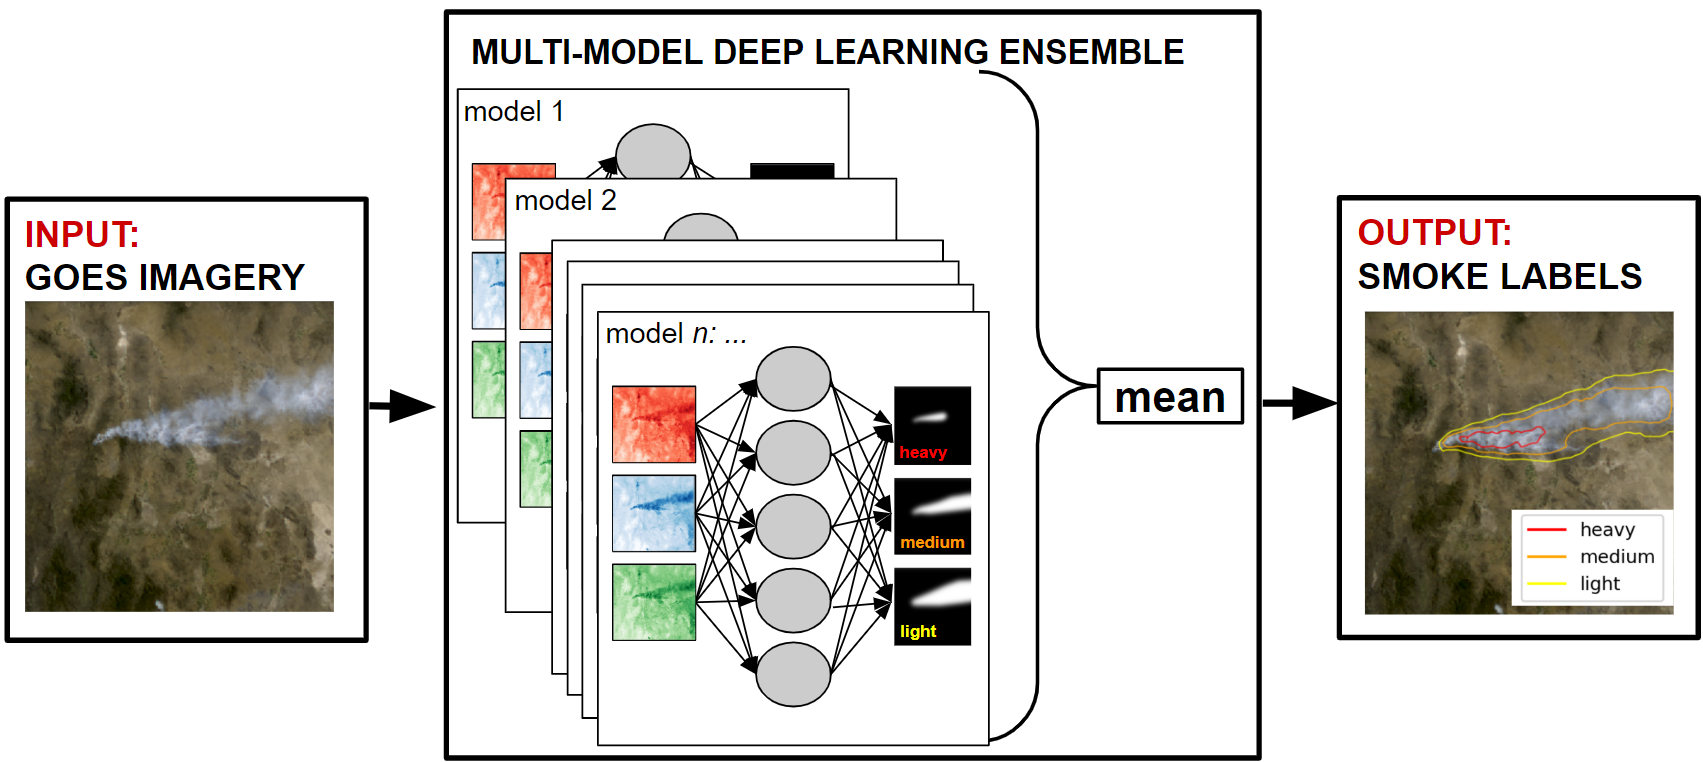
\includegraphics[width=0.7\textwidth]{ensemble_framework.png}
%     \caption{Multi-Model Ensemble Framework. GOES imagery is inputted to N independently-trained models whose output is combined with an unweighted average to produce the ensemble prediction of pixel-wise smoke labels.}
%     \label{fig:ensemble_framework}
% \end{figure}
\begin{SCfigure}[][h]
    \centering
    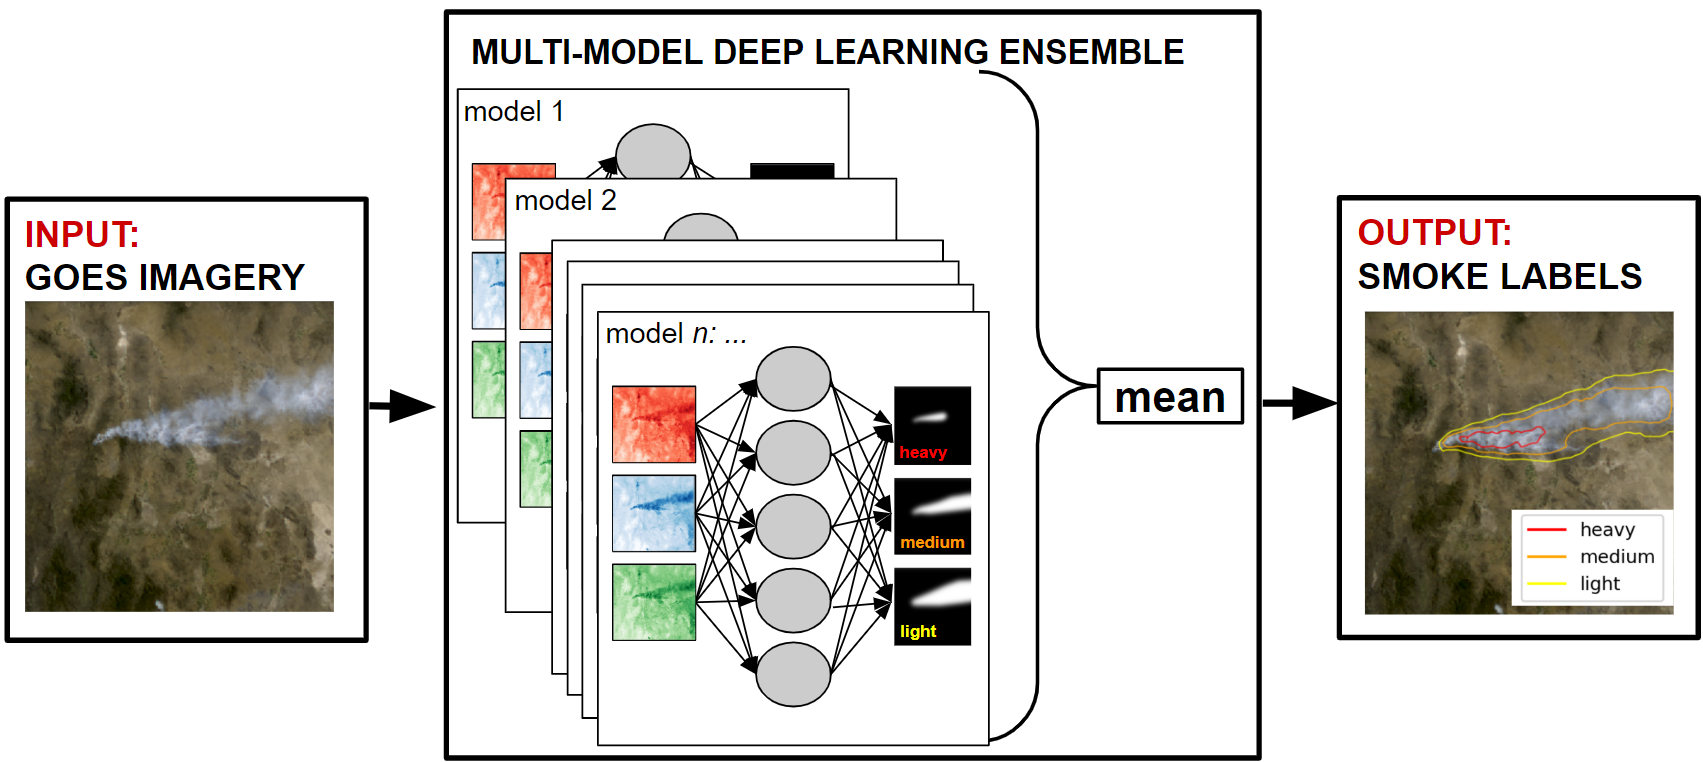
\includegraphics[width=0.7\textwidth]{ensemble_framework.png}
    \caption{\RaggedRight Multi-Model Ensemble Framework. GOES imagery is inputted to N independently-trained models whose output is combined with an unweighted average to produce the ensemble prediction of pixel-wise smoke labels.}
    \label{fig:ensemble_framework}
\end{SCfigure}
\section{Results}
Table \ref{tab:results} shows the IoU scores for individual models and ensembles. The ensemble of 8 different architectures outperforms the individual models, with an improvement in the IoU score over all densities and for each density individually. The ensemble of 8 models (with the same architecure, PAN) with different initial weights also outperforms the individual models, with a similar improvement in the IoU scores. Figure \ref{fig:ensemble_size_plot} shows the IoU performance over all smoke densities as a function of ensemble size for the two ensemble schemes. The ensemble of with different initial weights generally improves as models are added to the ensemble. This improvement is likely due to the different initializations leading to the models searching different parts of the parameter space and thus finding different minima of the loss function. The ensemble of different architectures improves with more models up to 8 models, but then starts to decrease in performance. This decrease in performance could be due to the additional architectures not being as well suited for the task, or the additional models not having enough variation in model bias to improve ensemble performance.
Figure \ref{fig:ensemble_panel} shows an example of smoke plume detection from the testing dataset. The ensemble predictions have smoother boundaries than the individual model outputs, making the prediction more comparable to the human-drawn polygon annotations.
\begin{table}[h]
    \centering
    \begin{tabular}{llrrr>{\bfseries}r}
        \hline
            &   Heavy &   Medium &   Light &   Overall \\
        \hline
         Single Model: DLV3P &   0.347 &     0.441 &  0.666 &      0.599  \\
         Single Model: PAN &  0.349 &     0.478 &  0.664 &      0.604 \\
        Architecture Ensemble (N=8) &   0.400 &     0.507 &  0.692 &      0.635 \\
        %  Architecture Ensemble (N=12) &  0.400 &     0.504 &  0.686 &      0.630 \\
        Random Initial Weights Ensemble (N=8) &  0.409 &     0.512 &  0.684 &      0.631 \\
        %  Random Initial Weights Ensemble (N=12) &   0.409 &     0.515 &  0.690 &      0.635 \\
         \hline
    \end{tabular}
    \caption{IoU results across three classes of smoke (light, medium, heavy) and over all densities. Presented for different individual models of different architectures (\citep{dlv3p}; \citep{PAN}), along with the archiecture-based ensemble and random initial weights ensemble performance, where N denotes the number of models in the ensemble.}
    \label{tab:results}
    \end{table}
% \begin{figure}[h]
%     \centering
%     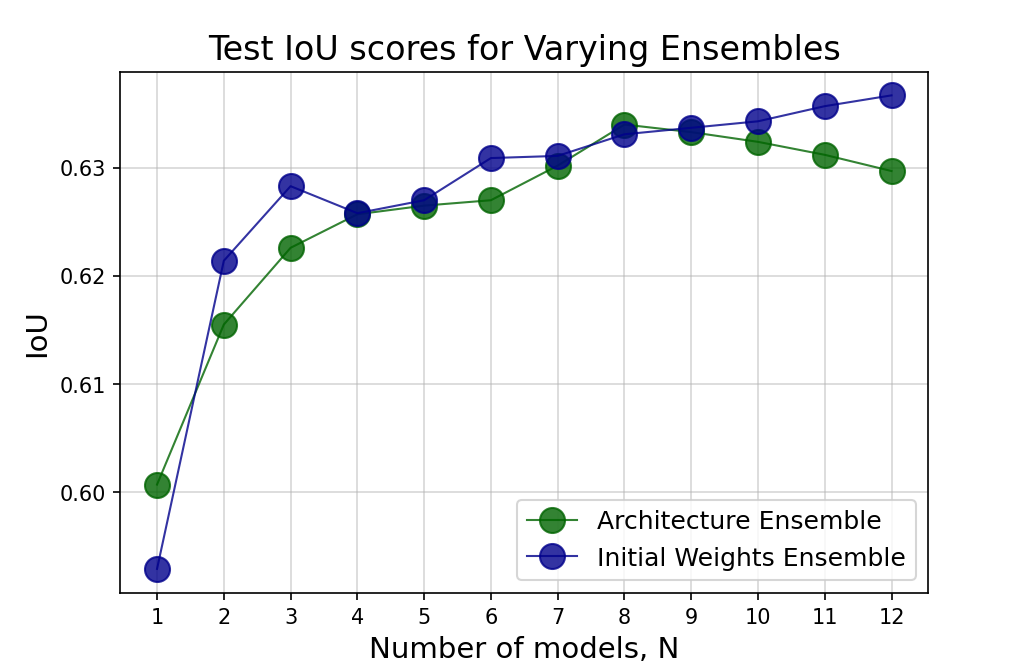
\includegraphics[width=0.70\textwidth]{ensemble_size_plot.png}
%     \caption{Ensemble IoU over all smoke densities as a function of ensemble size for two ensemble design schemes: random initial weights (blue) and architecure-based (red).}
%     \label{fig:ensemble_size_plot}
% \end{figure}
\begin{SCfigure}[][h]
    \centering
    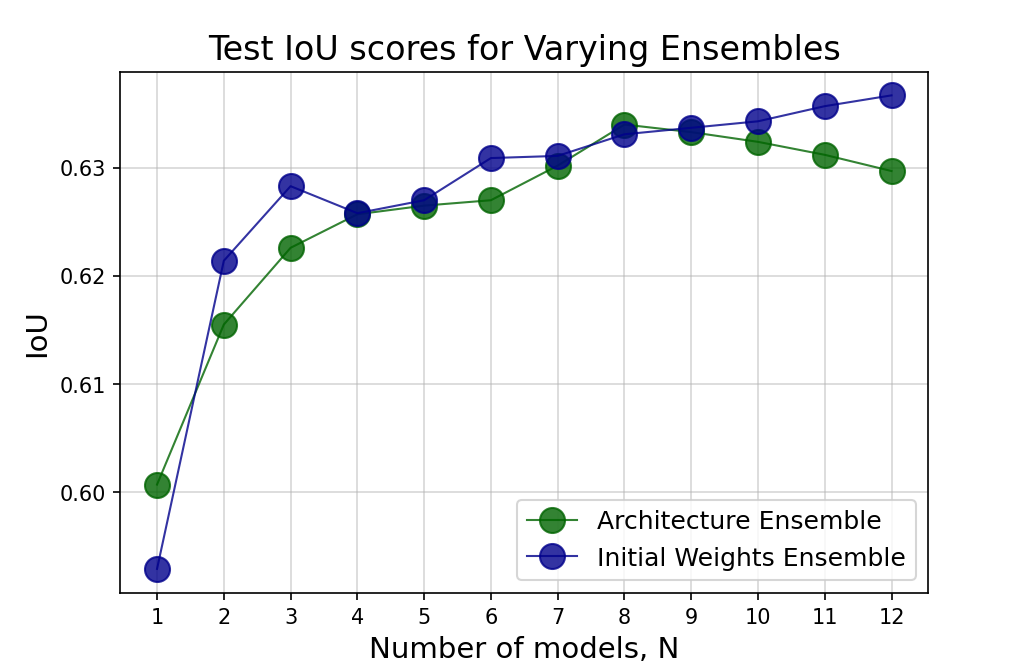
\includegraphics[width=0.70\textwidth]{ensemble_size_plot.png}
    \caption{\RaggedRight Ensemble IoU over all smoke densities as a function of ensemble size for two ensemble design schemes: random initial weights (blue) and architecure-based (red).}
    \label{fig:ensemble_size_plot}
\end{SCfigure}
\begin{figure}[h]
    \centering
    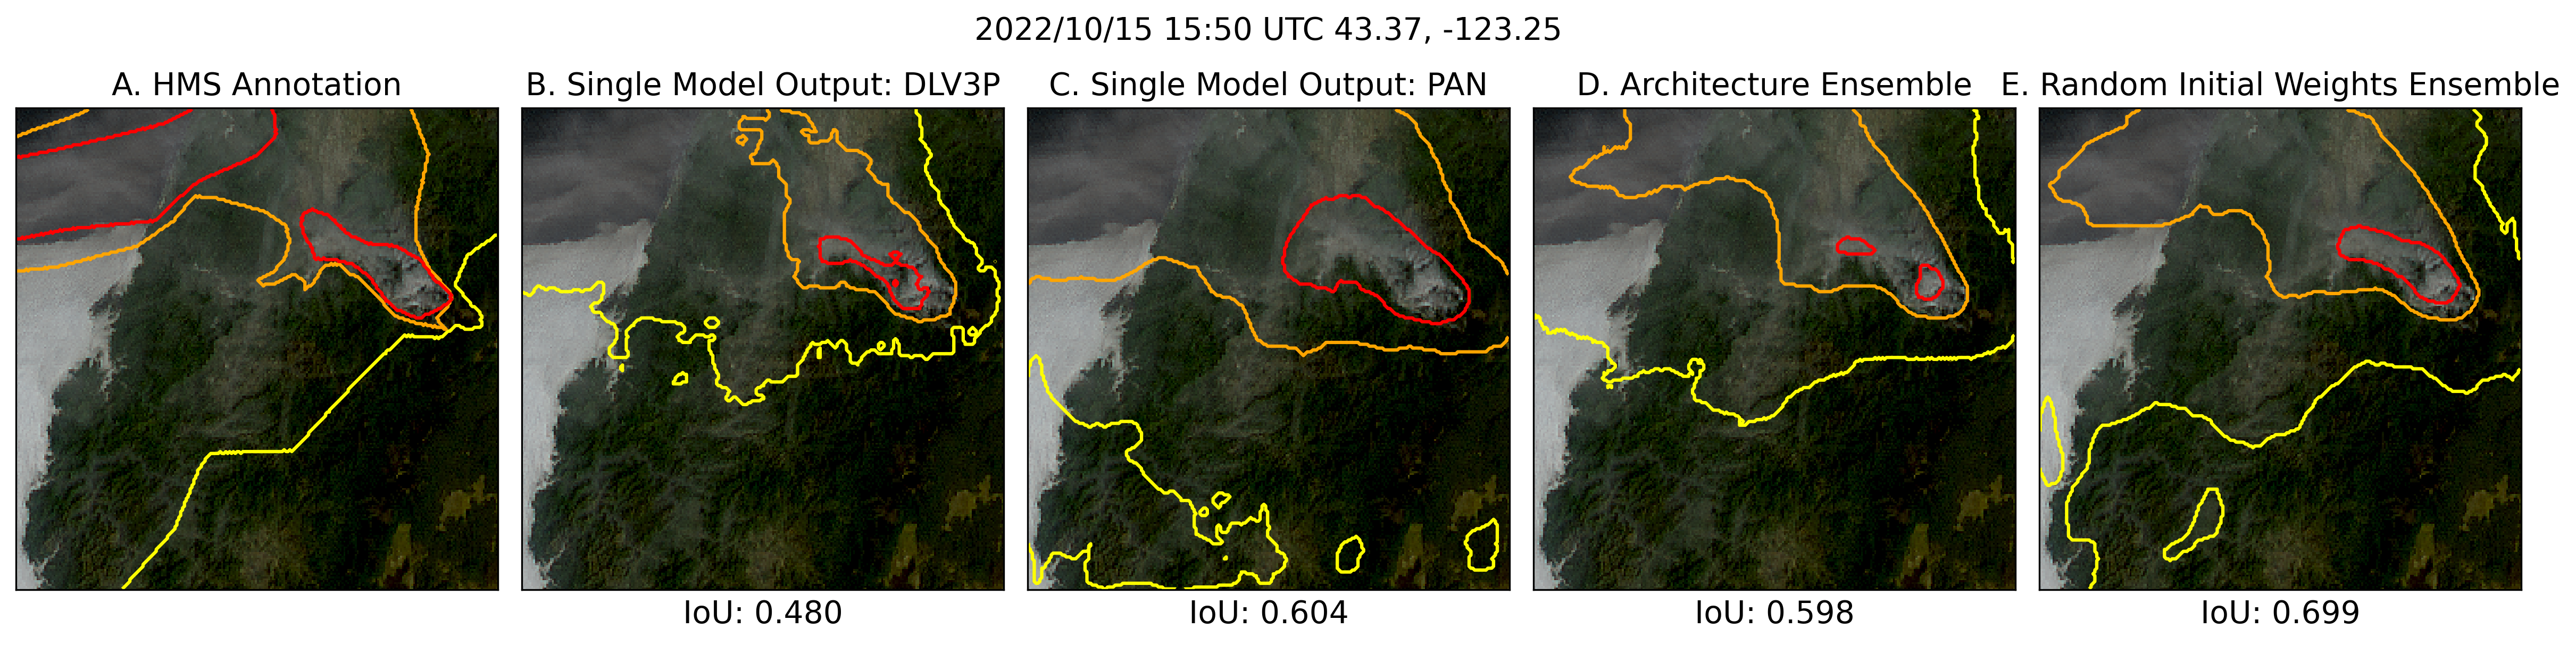
\includegraphics[width=\textwidth]{ensemble_panel_tinypaper.png}
    \caption{Example of smoke plume detection at (43.37, -123.25) on 2022/10/15 15:50 UTC. Red contours outline the heavy density smoke, orange contours outline the medium density smoke, and yellow contours outline the light density smoke annotations. Panel A displays the ground truth annotation; Panels B-C show the predictions of two individual models; Panel D shows the prediction of an architecture-based ensemble (N=8); Panel E shows the prediction of an ensemble (N=8) made with models initialized with different random weights.}
    \label{fig:ensemble_panel}
\end{figure}
\section{Conclusions and Future Work} We explore two schemes for building ensembles of deep learning models that both improve on testing set IoU and smooth annotation boundaries. However, further investigation is required to understand why the architecture-based ensemble decreases in performance after 8 models, and how an ensemble of both multiple architectures and different initial weights may perform. Also, we are experimenting with regionally-trained models, to further improve smoke detection. In the future, the application of these ensemble techniques are expected to aid in fire and hazard management by automating the monitoring of smoke in real-time from satellite imagery, ultimately supporting climate resilience and adaptation strategies. 
% This tool can be used to provide more frequent and consistent detection of smoke plumes
\bibliographystyle{plainnat}
\bibliography{references}
% Tips for Submissions (from CCAI site):
% For examples of typical formatting and content, see submissions from our previous workshops.
% Be explicit: Describe how your proposed approach addresses climate change, demonstrating an understanding of the application area.
% Frame your work: The specific problem and/or data proposed should be contextualized in terms of prior work.
% Address the impact: Describe the practical implications of your method in addressing the problem you identify, as well as any relevant societal impacts or potential side-effects. We recommend reading our further guidelines on this aspect here.
% Explain the ML: Readers may not be familiar with the exact techniques you are using or may desire further detail.
% Justify the ML: Describe why the ML method involved is needed, and why it is a good match for the problem.
% Avoid jargon: Jargon is sometimes unavoidable but should be minimized. Ideal submissions will be accessible both to an ML audience and to experts in other relevant fields, without the need for field-specific knowledge. Feel free to direct readers to accessible overviews or review articles for background, where it is impossible to include context directly.
% Addressing Impact
% Tackling climate change requires translating ideas into action. The guidelines below will help you clearly present the importance of your work to a broad audience, hopefully including relevant decision-makers in industry, government, nonprofits, and other areas.
% Illustrate the link: Many types of work, from highly theoretical to deeply applied, can have clear pathways to climate impact. Some links may be direct, such as improving solar forecasting to increase utilization within existing electric grids. Others may take several steps to explain, such as improving computer vision techniques for classifying clouds, which could help climate scientists seeking to understand fundamental climate dynamics.
% Consider your target audience: Try to convey with relative specificity why and to whom solving the problem at hand will be useful. If studying extreme weather prediction, consider how you would communicate your key findings to a government disaster response agency. If analyzing a supply chain optimization pilot program, what are the main takeaways for industries who might adopt this technology? To ensure your work will be impactful, where possible we recommend co-developing projects with relevant stakeholders or reaching out to them early in the process for feedback. We encourage you to use this opportunity to do so!
% Outline key metrics: Quantitative or qualitative assessments of how well your results (or for proposals, anticipated results) compare to existing methods are encouraged. Try to give a sense of the importance of your problem and your findings. We encourage you to convey why the particular metrics you choose are relevant from a climate change perspective. For instance, if you are evaluating your machine learning model on the basis of accuracy, how does improved accuracy on a machine learning model translate to climate impact, and why is accuracy the best metric to use in this context?
% Be clear and concise: The discussion of impact does not need to be lengthy, just clear.
% Convey the big picture: Ultimately, the goal of Climate Change AI is to “empower work that meaningfully addresses the climate crisis.” Try to make sure that from the beginning, you contextualize your method and its impacts in terms of this objective
% In this case, IoU is the best metric because it directly reflects the model's ability to correctly identify smoke plumes, which is essential for making informed decisions in real-time scenarios.
% would omit iou but want to address the following: also dont want to throw numbers at people with no explanation, but am short on space. should i add the equation??? ***
% workshop site: Outline key metrics: Quantitative or qualitative assessments of how well your results (or for proposals, anticipated results) compare to existing methods are encouraged. Try to give a sense of the importance of your problem and your findings. We encourage you to convey why the particular metrics you choose are relevant from a climate change perspective. For instance, if you are evaluating your machine learning model on the basis of accuracy, how does improved accuracy on a machine learning model translate to climate impact, and why is accuracy the best metric to use in this context?
% should i include this, to pertain to the climate change workshop? do i have room??? *** both these studies sitck to Western US
% Anthropogenic climate change drives warmer, drier conditions, leading to increased risk of severe wildfires \citep{cc-fire} \citep{climate-fire-risk}.
% from CCAI site: Each submission should make clear why the application has (or could have) a pathway to positive impacts regarding climate change.
% from CCAI site: Authors should clearly illustrate a pathway to climate impact, i.e., identify the way in which this work fits into broader efforts to address climate change. 
\end{document}